\chapter{Desarrollo del SITEM}

El presente capítulo presenta algunos aspectos relativos al desarrollo de los componentes principales del SITEM - figura \ref{arquitectura_sitem}. Formula lineamientos básicos a los diferentes grupos de desarrollo pero, teniendo en cuenta que el proyecto se adhiere al manifiesto de los metodólogos “ágiles”, lo que sigue es tan solo una recomendación y cada grupo lo enriquece con sus propias experiencias. 

\begin{figure}
 \centering
 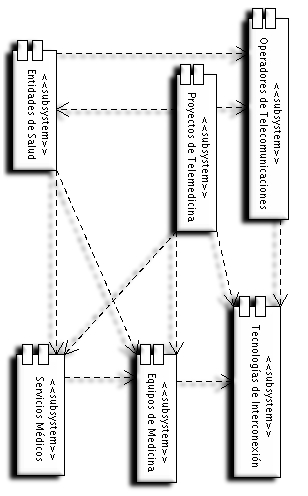
\includegraphics[width=108mm, height=174mm]{ArquitecturaGeneral.png}
 \caption{Subsistemas principales del SITEM}
 \label{arquitectura_sitem}
\end{figure}
\section{Modelos de Desarrollo del SITEM}

Para la implementación del Sistema de Información en Telemedicina se siguen las fases de desarrollo contempladas en el Proceso Unificado y se desarrollan los flujos de trabajo en las disciplinas básicas de:
\begin{itemize}
 \item Requisitos.
\item Análisis.
\item Diseño.
\item Elaboración.
\item Pruebas.
\end{itemize}

En cada fase se presentan resultados que permiten medir constantemente los avances en el proyecto, así como comprobar los niveles de calidad y la validez del método empleado. A partir de iteraciones continuas por las diferentes disciplinas se refinan constantemente los modelos.

\subsection{Modelo de Requisitos}

Los grupos de desarrollo en el SITEM\footnote{Cualquier nodo de desarrollo está a cargo de lo que se denomina genéricamente un \textit{grupo de desarrollo}. En general, un grupo de desarrollo en el SITEM no tiene un número de contribuyentes conocido.} deberán declarar explícitamente el concepto que da génesis a los diferentes componentes que desean abordar. Dicha declaración deberá ser coherente con los objetivos del SITEM y la filosofía del software libre, respetando siempre los principios constitucionales, la propiedad intelectual y el respeto al trabajo de los demás.

\subsubsection{Declaración del Problema}
Aunque en el ámbito colombiano como internacional existen estudios ampliamente conocidos acerca de la telemedicina, sus características, requerimientos, implicaciones y normatividad \cite{aparicio2003} \cite{bashshur77} \cite{bashshur95} \cite{oas2002}, la mayoría de ellos se encuentran disgregados y en idiomas diferentes al español por lo cual su consulta es compleja y no existe un mapa seguro de navegación que guíe al investigador hacia las fuentes confiables de información y este termina reinventando la rueda o, en el mejor de los casos, realizando un filtro interminable de información en donde lee, analiza y descarta datos – todo este trabajo tirado a la basura cuando otro investigador entra en escena y por falta de medios de socialización desconoce el trabajo del primero, iniciando un nuevo proceso.

Datos básicos de enlaces, grupos de investigación, proyectos e información técnica en telemedicina ha sido consignada en sendas tesis que, aunque completas en el estudio, no ofrecen la pertinencia y eficacia necesaria para el ambiente investigativo. 

La idea de integración de una \textit{comunidad de práctica investigativa} en el área de la telemedicina, perseguida durante varios años por la comunidad académica, ha sido torpedeada constantemente por los intereses comerciales de las empresas que ven en esta tecnología un beneficio meramente económico y no conciben un sistema de información integral abierto de caracter social por lo que promuevan la cultura del “ocultismo” de información propia de los procesos capitales. Estudios abandonados, e inconclusos, junto con la complejidad innecesaria del proceso de determinación del estado del arte, están abocando a los grupos universitarios a competir codo a codo - a pesar de todas sus limitaciones - contra grandes empresas multinacionales interesadas en “sacar del camino” a estos facilitadores de procesos.

Ante esta perspectiva la academia, cuya arma más tenaz es el conocimiento filosófico guiado por el método científico, debe propender por colectivizar eficaz y eficientemente todos sus avances en el campo de la telemedicina brindando alternativas públicas y de alta calidad. Es en esta tarea en la cual las tecnologías de la información entran a jugar un papel importante y más aún el medio de difusión más democrático, o anárquico si se quiere, que haya concebido la humanidad: \textit{Internet}. El Sistema de Información en Telemedicina debe hacer uso de dichas tecnologías y nacer como respuesta a las necesidades de información confiable, pertinente, eficaz y eficiente de la comunidad investigativa así como de mecanismos rápidos de socialización y actualización de resultados.

\subsubsection{Responsabilidades del Sistema}
El Sistema de Información en Telemedicina debe ser una herramienta de apoyo al investigador en el área de desarrollo de proyectos de Telemedicina. Para esto deberá estar, como mínimo, en capacidad de:

\begin{itemize}
\item \textbf{Gestionar la información y conocimiento de diferentes nodos declarados en una red de telemedicina.} se hace especial énfasis en los siguientes componentes ya caracterizados: entidades de salud, servicios médicos - incluyendo medicamentos y enfermedades, grupos de investigación en telemedicina, tecnologías de interconexión y operadores de telecomunicaciones.

\item \textbf{Administrar en forma segura los diferentes actores del sistema} para brindarles una experiencia enriquecida al interactuar con el Portal. La administración debe ser transparente y con miras a la estructuración avanzada de contenidos de acuerdo al perfil del usuario.

\item \textbf{Proveer instrumentos} para implementar metodologías de captura de información.

\item \textbf{Presentar la información} requerida por los actores enriqueciéndola con contenidos relacionados y haciendo uso de una GUI multimedia basada en tecnologías web.

\item \textbf{Integrar aplicaciones de software libre} que brinden funcionalidad de apoyo a las comunidades de práctica que se generen y fomente las tareas de capturar, extraer, organizar, analizar, encontrar, sintetizar, distribuir y compartir información y conocimiento. 

\item \textbf{Funcionar sobre una plataforma tecnológica basada en aplicaciones de software libre.}

\end{itemize}


\subsubsection{Definición de Alcances}

El SITEM es principalmente \textit{un concepto}, su estado actual es una representación del potencial real del sistema que debe ser socializado y entregado a la comunidad. La base de desarrollo principal es el grupo GITEM y será responsable de la versión oficial del producto. Sin embargo, dada la dinámica en el mundo del software libre, el grupo GITEM no limitará el trabajo independiente que sobre su desarrollo realice cualquier persona o grupo de personas. En este sentido la funcionalidad original del sistema podrá ser modificada pero no avalada directamente por el grupo.\footnote{Salvo en casos en que no se trasgredan directamente los objetivos primarios del desarrollo. En tales casos las contribuciones serán asociadas al hilo oficial de desarrollo.}. 

El SITEM ha sido creado con el fin de apoyar a los grupos de trabajo que realizan labores en el área de proyección de sistemas de telemedicina. La información que en él se encuentra debe ser ingresada por personas autorizadas para asegurar en un alto grado la veracidad e idoneidad de la misma. Sin embargo no se puede garantizar, y no se garantiza, la exactitud, disponibilidad, integridad y oportunidad de dicha información: \textit{la información contenida en el sitem no es una fuente oficial de datos}. El uso de la misma es responsabilidad de quien lo realiza. La información que se encuentre en el SITEM no ha sido necesariamente revisada por expertos profesionales. Todos los contenidos que se ingresen al SITEM deben ser de licencia pública o de libre uso; los contenidos que no cumplan estos criterios serán eliminados.

\subsubsection{Definición de actores}

El SITEM por su complejidad debe gestionar varios tipos de usuarios, cada uno con características específicas. Este tratamiento especial tiene que ver con el mantenimiento de la integridad de la información, la cual solo puede ser gestionada por un grupo selecto de usuarios. 

Algunos actores esperados en el SITEM son:

\begin{itemize}
\item Administrador.
\item Consultor.
\item Especialista Médico.
\item Profesional TIC.
\item Usuario General.
\end{itemize}

Cada uno de ellos con las características mostradas en el anexo \ref{modelo_requisitos}.

\subsubsection{Casos de uso}

Los requisitos funcionales del SITEM son declarados en diferente nivel de detalle por medio de una especificación de casos de uso, diagramas de comportamiento y de interacción. Como mínimo, al caracterizar un flujo de eventos por medio de un caso de uso se espera tener información acerca de:

\begin{itemize}
\item Nombre del Caso de Uso
\item Objetivo que se logra al ejecutarse el caso de uso.
\item Código que lo identifique unívocamente dentro del banco de artefactos.
\item Actores que intervienen al desarrollarse el caso de uso.
\item Casos de uso con los que está relacionado.
\item Precondiciones.  El estado del sistema que debe asegurarse antes de que el caso de uso inicie. Debido a que es responsabilidad del sistema no se verifica en el caso de uso.
\item Postcondiciones. Las características y estado del sistema una vez se haya terminado el caso de uso.
\item Flujo de Tareas. Flujo principal y alternativos de las tareas que se suceden al ejecutarse el caso de uso. Siempre se debe propender por mantener claridad en el modelo por lo que se recomienda utilizar diferentes artefactos para los flujos alternativos cuando esto lo amerite.
\end{itemize}

La tabla \ref{casouso}, muestra el caso de uso de diseño correspondiente al flujo principal del registro de un usuario en el sistema.

\begin{table}
\begin{center}
\begin{tabular}{|l|p{10cm}|}
\hline
\textbf{Caso de Uso}&\\
\hline
Nombre & Registrarse en el SITEM\\
\hline
Objetivo & El actor logra crear una cuenta en el SITEM con un rol específico para poder trabajar en un subsistema dado.\\
\hline
Código Interno & UC-GENERAL-001 \\
\hline
Actores & Usuario General\\
\hline
Precondiciones & Ninguna.\\
\hline
Flujo Básico & 1. El usuario general selecciona la opción de nuevo usuario desde la página principal del SITEM.\\
& 2. El SITEM muestra un formulario con los campos:\\
& Nombres\\
& Apellidos\\
& Correo Electrónico\\
& Teléfono\\
& Nombre de Usuario\\
& Clave\\
& Reescriba la clave\\
& Acceso Requerido\\
& 3. El usuario diligencia uno a uno los campos requeridos y opcionales.\\
& 4. El usuario envía los datos al SITEM.\\
& 5. El SITEM verifica que los datos tengan los formatos esperados.\\
& 6. El SITEM ingresa el registro a la base de datos colocando el campo de estado en 1 - registrado sin autorización.\\
& 7. El SITEM redirecciona a la página de registro exitoso.\\
& 8. El usuario acepta el mensaje.\\
\hline
Postcondiciones & Se agregó un registro en la base de datos con el campo de estado en 1.\\
\hline
Casos de uso relacionados&Seleccionar Rol en el SITEM\\
\hline
\end{tabular}
\caption{Caso de Uso Registrarse en el SITEM}
\label{casouso} 
\end{center}
\end{table}

El modelo de casos de uso consta en la actualidad con 180 elementos principales definidos\footnote{No se incluyen casos de uso implementados en aplicaciones conexas.} y más de 230 flujos alternativos - los más relevantes incluidos en el anexo \ref{modelo_requisitos}. Con esto se concreta los requerimientos de autenticación, gestión de información - incluyendo generaciones de informes, trabajo en grupo, consultoría y georeferenciación. Muchos de ellos aún no se han desarrollado en su totalidad por lo que se preve que este modelo sufra modificaciones.

\subsection{Modelo de Análisis y Diseño}

El modelo de requisitos es insumo para modelar los componentes del sistema con los modelos de análisis - en donde se especifica en más detalle cada caso de uso; y el de diseño, en donde se modela el comportamiento y la estructura de los diferentes componentes que implementarán la funcionalidad. Deliberadamente se unen estas dos disciplinas en un solo modelo para evitar un excesiva concentración de documentación en el análisis.

El equipo de desarrollo se ha apoyado en diferentes diagramas de estructura, de comportamiento e interacción. El anexo \ref{modelo_analisis} corresponde al modelo de análisis y diseño conteniendo los elementos más interesantes para diferentes componentes del sistema. En este punto cobra importancia la aplicación de ciertos patrones GRASP \cite{larman2003} especialmente se presta atención a mantener los principios de:

\begin{itemize}
\item Alta Cohesión
\item Bajo Acoplamiento
\end{itemize}

Asignando responsabilidades teniendo en cuenta:
\begin{itemize}
\item Experto en Información.
\item Controlador
\end{itemize}

En la figura \ref{secuencia}, se muestra el diagrama de interacción correspondiente a la realización del caso de uso registrarse en el sistema.

\begin{figure}
 \centering
 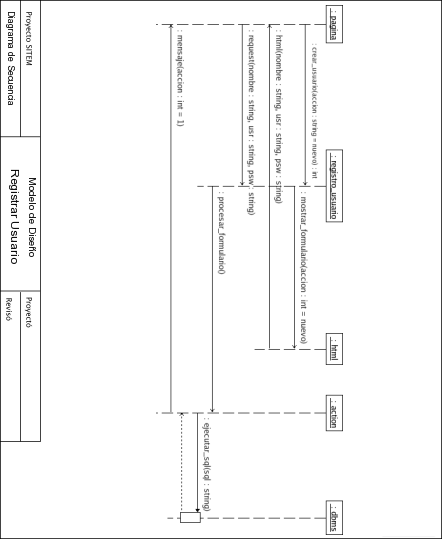
\includegraphics[width=156mm, height=156mm]{secuencia.png}
 \caption{Realización del Caso de Uso registrarse en el Sistema}
 \label{secuencia}
\end{figure}


\subsection{Modelo de Implementación}

El conjunto de diagramas del Anexo \ref{modelo_analisis} brinda la información fundamental para el modelo de implementación. En el SITEM se agrupan los diferentes componentes en la jerarquía de carpetas mostrada en la figura \ref{carpetas_sitem}.

Cada una de las carpetas contiene los ficheros de código fuente del producto:

\begin{itemize}
 \item \textbf{Clases:} Contiene los archivos en PHP que implementan las clases. 
\item \textbf{Funciones:} Grupo de funciones en JavaScript para la validación de información en el nodo de usuario. En la actualidad la fase IV contempla complementar esta aproximación con la utilización de AJAX.
\item \textbf{Configuración:} Alberga el archivo \textit{config.inc.php} que guarda las variables de ingreso a la base de datos. Dichas variables se encuentran codificadas de acuerdo al algoritmo que se seleccione (o implemente) desde la clase \textit{codificar}.
\item \textbf{Bloques:} Agrupa el código fuente de cada bloque desarrollado en el SITEM. Un bloque se define como una unidad de funcionalidad independiente que puede utilizarse en cualquier página.
\item \textbf{Estilo:} Información acerca de los parámetros generales de estilo - tamaño de fuente, color de bordes, fondos, colores de letras, etc; para diferentes componentes del SITEM. La modificación o inclusión de parámetros afectará la interfaz global del sistema. Actualmente los estilos en el SITEM se basan en hojas de estilo CSS.
\item \textbf{Gráficos:} Todos los archivos gráficos usados en el proyecto.
\item \textbf{Documentos:} Carpeta inicialmente vacía que se utiliza para guardar los archivos que los usuarios caragen a través del protocolo HTTP. Por seguridad se recomienda que esta carpeta se encuentre fuera del directorio en donde se encuentra instalada la aplicación.
\item \textbf{Instalar:} Contiene el instalador del producto. Esta carpeta debería ser retirada una vez el sitio se encuentre en producción.
\item \textbf{Desarrollo:} Con varios scripts que facilitan la tarea de desarrollo y adaptación de bloques en el sistema. Estos scripts se han construidos pensando en plataformas de desarrollo y prueba por lo que se supone no debe encontrarse en plataformas de producción.
\end{itemize}

En todo caso, durante el proceso de instalación se puede - y recomienda; asociar nuevos nombres a las carpetas por lo que en teoría ningún desarrollo basado en el SITEM que esté en etapa de producción debería tener nombres de carpetas conocidos.

\begin{figure}
 \centering
 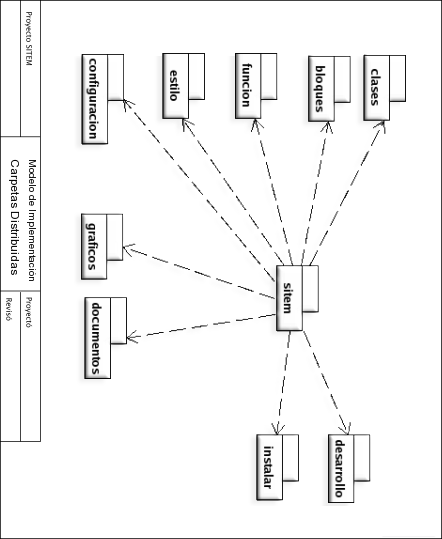
\includegraphics[width=156mm, height=156mm]{carpetas.png}
 \caption{Carpetas que se distribuyen con el SITEM}
 \label{carpetas_sitem}
\end{figure}

\subsubsection{Acerca de la Seguridad}
El uso lenguajes de scripts en el lado del servidor puede tener algunos problemas de seguridad cuando son accedidos mediante instrucciones tipo GET - inserción SQL, data binding, etc: por esta razón cuando se usan variables usando este método todas se cifran en una cadena combinada de 256 bits, figura \ref{desenlace}. Todas las peticiones desde el cliente se realizan usando métodos POST sin perjuicio de la funcionalidad. Se prefiere sobre cualquier otro criterio el manejo de cookies pero en el caso de que estas estén deshabilitadas toda la información se validará empleando la dirección IP inicial de conexión.

En cuanto a la integridad de los datos se tiene un modelo de comparación de contenidos que se activa cada periodo de tiempo, el cual es programable; proponiéndose mantener una copia de respaldo verificada y avalada por el administrador. En caso de corrupción o pérdida de datos se mantiene una lista completa de los usuarios del sistema de hasta 1'000.000 de sesiones de tipo desplazamiento en donde el usuario más antiguo es descartado para la inclusión del nuevo cuando el tamaño asignado es completado, asegurándose así el manejo eficiente de disco.

Por ningún motivo se permite el acceso a sitios restringidos a usuarios que no hayan sido plenamente identificados en el sistema. En sitios críticos se hace una revisión de los datos de acceso guardados en cookies o se constata los datos de inicio de sesión. Se han evitado al máximo los usos de carácter comodín y todos los accesos a la base de datos son validados en su sintaxis. El SITEM actualmente propone el uso de protocolos seguros tales como SSL o SHTML.

Vale la pena destacar el uso de metodologías de autenticación de usuario basado en sesiones y codificación de datos que permiten ofrecer un contenido personalizado de acuerdo al perfil de cada uno de los clientes del sistema.

\begin{figure}
 \centering
 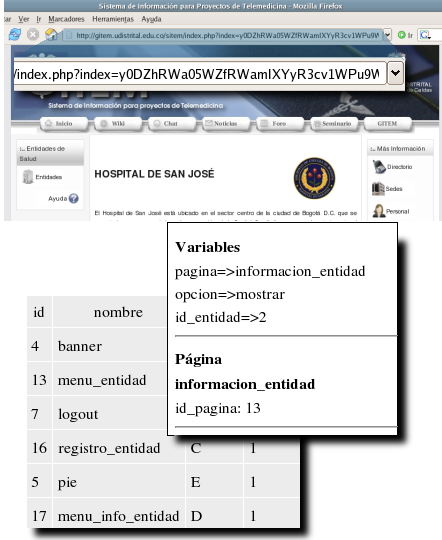
\includegraphics[width=156mm, height=156mm]{desenlace.png}
 \caption{URL encriptada. Con la herramienta \textit{Desenlace} el desarrollador puede descifrar los datos}
 \label{desenlace}
\end{figure}


\subsection{Modelo de Datos}

Dentro del proceso de desarrollo del SITEM el modelado y elaboración del sistema de bases de datos es una de las partes fundamentales de la propuesta. Se ha venido estructurando el modelo de acuerdo a las necesidades de cada módulo en particular para garantizar la independencia entre ellos en cada una de las capas, incluyendo la de persistencia.

Dependiendo de las caracterísitcas de cada subsistemas se implementan o no políticas transaccionales. El modelo de seguridad en los datos hereda todos los elementos del servidor tales como bloqueos de puertos, ocultación de ventanas, manejo de sockets, etc; además, un esquema lógico de validación por conexiones persistentes complementa estas características.

El anexo \ref{modelo_datos} contiene los diagramas de clases que describen la arquitectura de datos del sistema y cada uno de sus subsistemas asociados. 

En la actualidad el SITEM acepta bases de datos PostgreSQL, MySQL y ORACLE. La capa de persistencia del hilo principal se despliega sobre un servidor MySQL 5.0.27-standard.


\subsection{Interfaz gráfica.}

De acuerdo a los diagramas conceptuales del portal GITEM y del SITEM. Se han utilizado para la creación de las páginas los conceptos de diseño web enumerado por (Maldonado,2001), intentando evitar al máximo las páginas sobrecargadas de información. La navegación es guiada mediante enlaces dentro de las mismas páginas las cuales están agrupadas temáticamente logrando una coherencia en el contenido. 

Los gráficos han sido optimizados y su inclusión es necesaria para dar ayuda visual al contenido basado en texto. Teniendo en cuenta que el SITEM esta diseñado para interactuar permanentemente y por periodos prolongados de tiempo con el cliente, se han evitado deliberadamente la utilización  de componentes dinámicos tales como películas en flash, gif animados o menús desplegables. No obstante, el diseño no pierde atractivo ya que su implementación se fundamenta en estudios técnicos de comportamiento humano cuando navegan por Internet.

Para reducir el tiempo de acceso al portal, sobre todo cuando se trabaja con conexiones lentas, se da la posibilidad en algunos subsistemas de descargar en formato PDF todo el contenido del grupo de páginas en donde se este ubicado.

\subsubsection{Arquitectura de la página}

Independiente del subsistema que nos encontremos las páginas siempre están compuestas por cinco secciones denominadas genéricamente con las letras A, B, C, D y E. En ellas se distribuyen los diferentes bloque que conforman la página en una arquitectura Top - Down. Las páginas que no tienen bloques en todas las secciones colapsan aquellas que no se utilizan para dar una impresión visual consistente. Las figuras \ref{secciones} y \ref{seccion_colapsada} muestran gráficamente el manejo de las secciones en cada página.

\begin{figure}
 \centering
 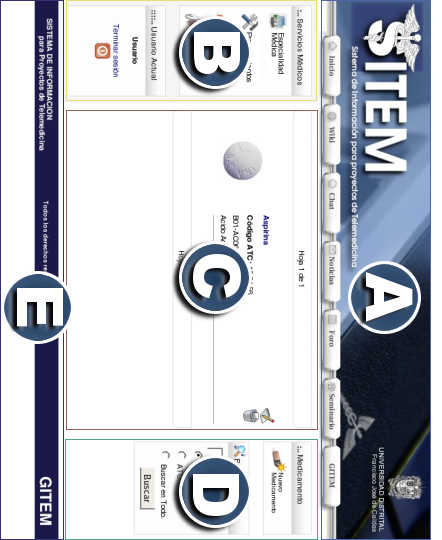
\includegraphics[width=156mm, height=156mm]{secciones.png}
 \caption{Arquitectura de una página en el SITEM}
 \label{secciones}
\end{figure}

\begin{figure}
 \centering
 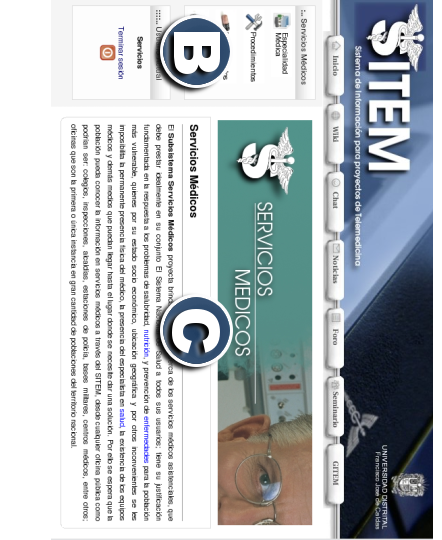
\includegraphics[width=156mm, height=156mm]{seccion_colapsada.png}
 \caption{Página del SITEM en donde la Sección D se ha colapsado.}
 \label{seccion_colapsada}
\end{figure}

\subsection{Entregables del proyecto}

Los siguientes artefactos – documentos, son generados y utilizados por el proyecto. Una copia de cada uno de ellos puede ser descargada desde Internet. \footnote{En una carpeta especialmente diseñada para esto: http://gitem.udistrital.edu.co/sitem/desarrollo/index.php.} En el anexo \ref{entregables} se tiene extractos importantes de algunos de ellos.

\begin{itemize}
\item \textbf{Plan General de Trabajo}
\item \textbf{Modelo de Casos de Uso}. El cual especifica los requerimientos que debe cumplir el módulo de software y que en últimas constituye los contratos que éste, el módulo, tiene con actores externos. Este artefacto estará hecho en su totalidad usando el Lenguaje de Modelado Unificado. 

Dentro de este modelo se tienen dos vistas claras: la del negocio y la del sistema. El modelo de Casos de Uso del Negocio ilustra el ámbito del negocio que esta siendo modelado. El diagrama contiene actores del negocio y los servicio o funciones que ellos requieren del negocio. El modelo de casos de uso del sistema representa el ámbito de una aplicación. De esto se tiene que un solo modelo de casos de uso del negocio puede tener muchos Modelos de casos de uso asociados, donde cada modelo de casos de uso representa una única aplicación.

\item \textbf{Modelo de Objetos.} El cual describe la forma en que cada requerimiento – o contrato,  es cumplido. Establece las entidades internas, la información que intercambian y los flujos de trabajo que logran el cumplimiento de los requisitos. Los grafos correspondientes podrán incluir diagramas estáticos o interactivos expresados en UML.

\item \textbf{Glosario.} Que es el único artefacto válido de consulta para la terminología usada en el desarrollo del SITEM. Ver el anexo \ref{glosario}.

\item \textbf{Visión.} Este documento define la visión del SITEM. Es de todos el que marca las pautas conceptuales. 

\item \textbf{Especificaciones Adicionales.} Este documento capturará todos los requisitos que no han sido incluidos como parte de los casos de uso y se refieren requisitos no-funcionales globales. Dichos requisitos incluyen: requisitos legales o normas, aplicación de estándares, requisitos de calidad del producto, tales como: confiabilidad, desempeño, etc., u otros requisitos de ambiente, tales como: sistema operativo, requisitos de compatibilidad, etc. 

\item \textbf{Prototipos de Interfaces de Usuario.} Se trata de prototipos que permiten al usuario hacerse una idea más o menos precisa de las interfaces que proveerá el sistema y así, conseguir retroalimentación de su parte respecto a los requisitos del sistema. Estos prototipos se realizarán como: dibujos a mano en papel, dibujos con alguna herramienta gráfica o prototipos ejecutables interactivos, siguiendo ese orden de acuerdo al avance del proyecto. Sólo los de este último tipo serán entregados al final de la fase de Elaboración, los otros serán desechados. Asimismo, este artefacto, será desechado en la fase de Construcción en la medida que el resultado de las iteraciones vayan desarrollando el producto final. 

\item \textbf{Modelo de Análisis y Diseño.} Este modelo establece la realización de los casos de uso en clases y pasando desde una representación en términos de análisis (sin incluir aspectos de implementación) hacia una de diseño (incluyendo una orientación hacia el entorno de implementación), de acuerdo al avance del proyecto.  Consultar el anexo \ref{modelo_analisis}.

\item \textbf{Modelo de Datos.} Previendo que la persistencia de la información del sistema será soportada por una base de datos relacional, este modelo describe la representación lógica de los datos persistentes, de acuerdo con el enfoque para modelado relacional de datos. Para expresar este modelo se utiliza un Diagrama de Clases (donde se utiliza un profile UML para Modelado de Datos, para conseguir la representación de tablas, claves, etc.). El anexo \ref{modelo_datos} contiene los artefactos más importantes del modelo de datos. 

\item \textbf{Modelo de Implementación.} Este modelo es una colección de componentes y los subsistemas que los contienen. Estos componentes incluyen: ficheros ejecutables, ficheros de código fuente, y todo otro tipo de ficheros necesarios para la implantación y despliegue del sistema.

\item \textbf{Modelo de Despliegue.} Este modelo muestra el despliegue la configuración de tipos de nodos del sistema, en los cuales se hará el despliegue de los componentes. Ver anexo \ref{modelo_despliegue} 

\item \textbf{Casos de Prueba.} Cada prueba es especificada mediante un documento que establece las condiciones de ejecución, las entradas de la prueba, y los resultados esperados. Estos casos de prueba son aplicados como pruebas de regresión en cada iteración. Cada caso de prueba llevará asociado un procedimiento de prueba con las instrucciones para realizar la prueba, y dependiendo del tipo de prueba dicho procedimiento podrá ser automatizable mediante un script de prueba. 

\item \textbf{Solicitud de Cambio.} Los cambios propuestos para los artefactos se formalizan mediante este documento. Mediante este documento se hace un seguimiento de los defectos detectados, solicitud de mejoras o cambios en los requisitos del producto. Así se provee un registro de decisiones de cambios, de su evaluación e impacto, y se asegura que éstos sean conocidos por el equipo de desarrollo. Los cambios se establecen respecto de la última baseline (el estado del conjunto de los artefactos en un momento determinado del proyecto) establecida. En nuestro caso al final de cada iteración se establecerá una baseline. 

\item \textbf{Plan de Iteración.} El conjunto de actividades y tareas se orden temporalmente y se le asignan recursos a corto plazo. Se realiza para cada iteración y en todas las fases. 

\item \textbf{Lista de Riesgos.} Este documento incluye una lista de los riesgos conocidos y vigentes en el proyecto, ordenados en orden decreciente de importancia y con acciones específicas de contingencia o para su mitigación. El anexo \ref{riesgos} contiene la declaración de los riesgos más importantes detectados en el proyecto así como estrategias para minimizarlos.

\end{itemize}